\section{Requisiti funzionali}
I requisiti funzionali sono stati esplicitati mediante il diagramma UML dei casi d’uso in \figurename~\ref{fig:use_cases_diagram}, il quale è composto da 4 attori (Amministratore, Cucina, Cassiere e Cliente che tramite ereditarietà viene ridefinito in Cliente al tavolo oppure Cliente che effettua ordinazioni d’asporto) e 6 viste (vista amministratore, vista cucina, vista cassiere, vista cliente, vista cliente al tavolo e sistema).

\begin{figure}[htbp]
	\begin{comment}
	The [htbp] option in LaTeX is used to fine-tune the placement of tables and figures.
	Each letter in [htbp] stands for a particular placement option:
	h (here): Place the table or figure in the text where the environment (like figure or table) is written, if there is enough room left on the page.
	t (top): Place it at the top of a page.
	b (bottom): Place it at the bottom of a page.
	p (page): Place it on a page containing only floats, such as figures and tables	
	LaTeX will try to place the float at the location that comes first in the option list.
	If it can’t place it there due to constraints like page size, it will move on to the next option. If none of the specified options work, LaTeX will hold the float until it finds a place where it fits, or until a \clearpage command is encountered
	\end{comment}
	\centering
	
	% verticale
	%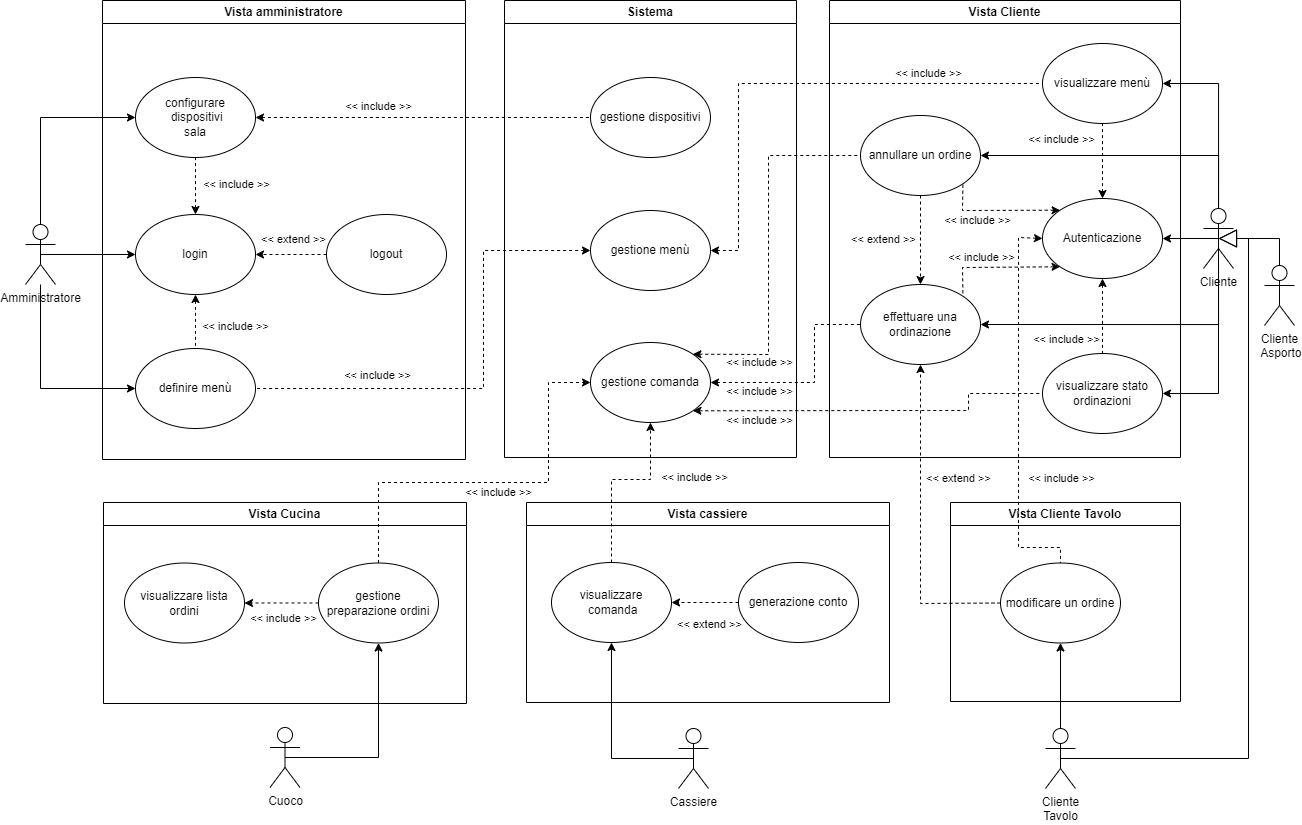
\includegraphics[scale=0.4, angle=90]{iterazione0/images/use_cases_diagram}
	
	% orizzontale
	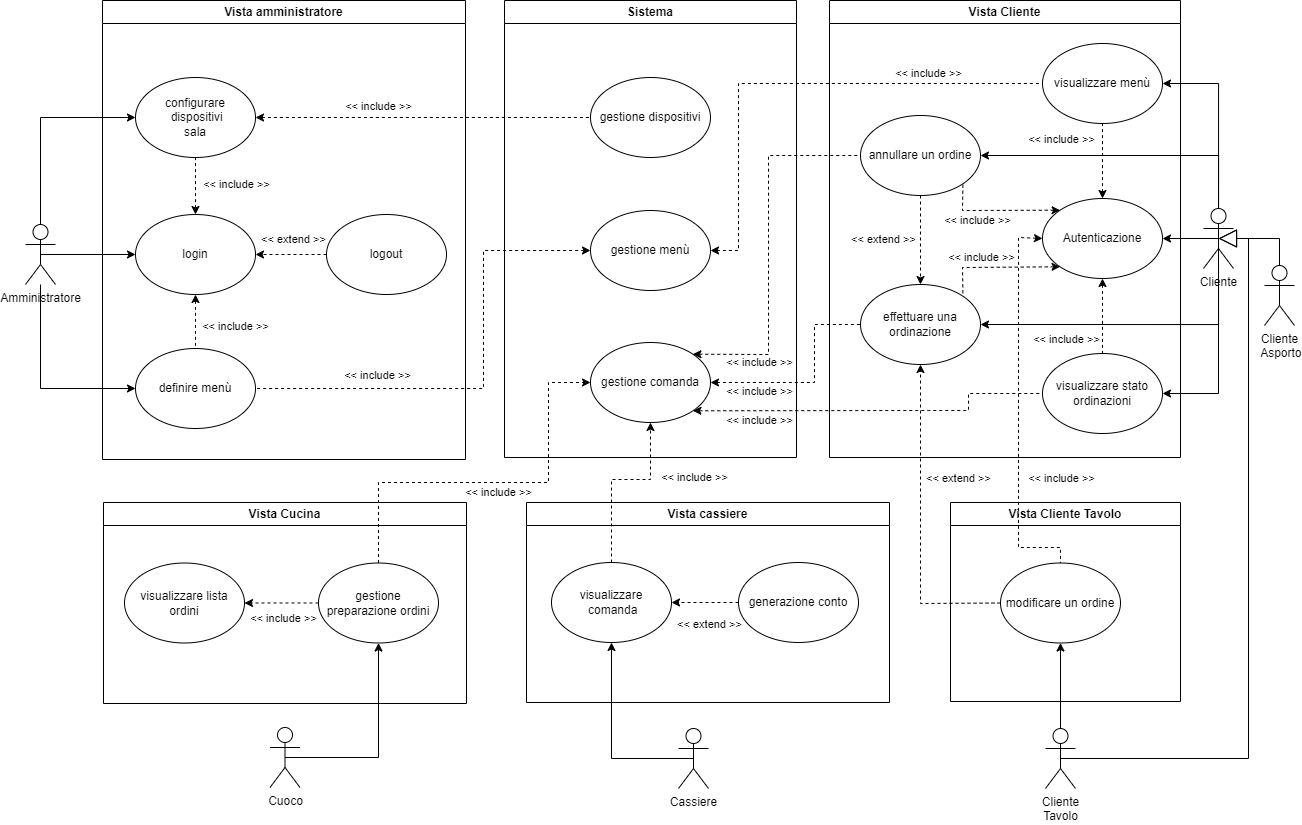
\includegraphics[scale=0.25]{iterazione0/images/use_cases_diagram}
	\caption{Diagramma dei casi d'uso\label{fig:use_cases_diagram}}
\end{figure}


Per ottimizzare il processo di sviluppo, si è deciso di categorizzare le specifiche funzionali in tabelle con tre livelli di priorità: elevata, media e bassa. Nello specifico il primo livello è assegnato alla Tabella~\ref{tab:use_cases_high_priority} a cui sono attribuiti i casi d'uso essenziali per il funzionamento dell'applicazione, i casi d'uso relativi alle funzionalità aggiuntive non critiche sono stati attribuiti alla Tabella~\ref{tab:use_cases_medium_priority} a priorità media, mentre il livello a bassa priorità che accoglie requisiti funzionali opzionali previsti per versioni successive alla Tabella~\ref{tab:use_cases_low_priority} .

\clearpage
\subsection{Priorità elevata}

\begin{table}[htbp]
	\centering
	 \begin{tabularx}{\textwidth}{|>{\centering\arraybackslash} m{4em}| >{\raggedright\arraybackslash}X |}
		\hline
		\textbf{Codice} & \textbf{Titolo} \\ [0.5ex]
		\hline\hline
		UC1 & Registrazione amministratore  \\
		\hline
		UC2 & Configurazione e gestione dispositivi (tavoli, cucina, cassa) \\
		\hline
		UC3 & Login/logout amministratore \\
		\hline
		UC4 & Gestione menù \\
		\hline
		UC5 & Algoritmo gestione coda ordini \\
		\hline
		UC6 & Cucina visualizza ordini da preparare \\
		\hline
		UC7 & Cucina notifica preparazione piatto \\
		\hline
		UC8 & Identificazione cliente \\
		\hline
		UC9 & Cliente visualizza menu \\
		\hline
		UC10 & Cliente effettua ordinazione \\
		\hline
		UC11 & Gestione sessione cliente \\
		\hline
		UC12 & Cassiere visualizza il conto \\
		\hline
	\end{tabularx}
	\caption{Casi d'uso ad elevata priorità}
	\label{tab:use_cases_high_priority}
\end{table}

\subsection{Priorità media}
\begin{table}[htbp]
	\centering
	\begin{tabularx}{\textwidth}{|>{\centering\arraybackslash} m{4em}| >{\raggedright\arraybackslash}X |}
		\hline
		\textbf{Codice} & \textbf{Titolo} \\ [0.5ex]
		\hline\hline
		UC13 & Modifica ordine al tavolo  \\
		\hline
		UC14 & Annullare un ordine \\
		\hline
		UC15 & Modifica priorità piatto (aumentare, diminuire) \\
		\hline
		UC16 & Cliente visualizza stato delle ordinazioni  \\
		\hline
	\end{tabularx}
	\caption{Casi d'uso a media priorità}
	\label{tab:use_cases_medium_priority}
\end{table}

\subsection{Priorità bassa}
\begin{table}[htbp]
	\centering
	\begin{tabularx}{\textwidth}{|>{\centering\arraybackslash} m{4em}| >{\raggedright\arraybackslash}X |}
		\hline
		\textbf{Codice} & \textbf{Titolo} \\ [0.5ex]
		\hline\hline
		UC17 & Identificazione cliente asporto  \\
		\hline
		UC18 & Cliente effettua ordinazione asporto  \\
		\hline
		UC19 & Gestione prioritaria ordinazioni da asporto \\
		\hline
		UC20 & Strategia greedy “a gruppi” (ingrediente principale in comune)   \\
		\hline
	\end{tabularx}
	\caption{Casi d'uso a bassa priorità}
	\label{tab:use_cases_low_priority}
\end{table}

\clearpage